\documentclass[t,aspectratio=169]{beamer}
%\usetheme{Berkeley}
\usepackage{graphicx}
\usepackage{amsmath}
\usepackage[american]{circuitikz}

\title{Clase 19}
\subtitle{El modelo de Ebers-Moll del BJT}
\author{Dr.-Ing. Juan José Montero Rodríguez}
\subject{Elementos Activos}
\institute{Escuela de Ingeniería Electrónica}
\date{Semestre II-2023}

\begin{document}

\begin{frame}{}
\maketitle
\end{frame}

\section{Ebers-Moll}
\begin{frame}{Modelo de Ebers-Moll NPN}

\vspace{-5mm}
\begin{columns}
\begin{column}{0.5\textwidth}

\begin{itemize}
    \item Modelo describe la operación de ambos diodos: $D_{BE}$ y $D_{BC}$.
    \item Permite encontrar el punto de operación en cualquiera de las regiones:
    \begin{itemize}
        \item Corte
        \item Activa directa
        \item Activa reversa
        \item Saturación débil
        \item Saturación fuerte
    \end{itemize}
    \item La dirección de las corrientes es muy importante, signo positivo siempre que la corriente entra al transistor.
    \item La suma de las tres corrientes es cero.
\end{itemize}

\end{column}
\begin{column}{0.5\textwidth}

\begin{figure}[H]
    \centering
    \begin{circuitikz}
        % diodos
        \draw (0,0) to[D,l_=$D_{BC}$,i=$I_R$] (2,0);
        \draw (0,0) to[D,l^=$D_{BE}$,i=$I_F$] (-2,0);
        % fuentes dependientes
        \draw (-2,2) to[cisource,l^=$\alpha_R I_R$] (0,2);
        \draw (2,2) to[cisource,l_=$\alpha_F I_F$] (0,2);
        % conexiones
        \draw (-2,0) -- (-2,2);
        \draw (0,0) -- (0,2);
        \draw (2,0) -- (2,2);
        \draw (-2,1) to[short,-o] (-2.5,1);
        \draw (-2.5,1) node[left] {$E$};
        \draw (2,1) to[short,-o] (2.5,1);
        \draw (2.5,1) node[right] {$C$};
        \draw (0,0) to[short,-o] (0,-0.5);
        \draw (0,-0.5) node[below] {$B$};
        % corrientes
        \draw[->] (-2.75,1.25) -- (-2.25,1.25);
        \draw[->] (2.75,1.25) -- (2.25,1.25);
        \draw[->] (-0.25,-0.75) -- (-0.25,-0.25);
    \end{circuitikz}
\end{figure}

\[ I_B + I_C + I_E = 0 \]

\[ \alpha_F I_{ES} = \alpha_R I_{CS} \]

\end{column}
\end{columns}

\end{frame}


\begin{frame}{Ecuaciones de Ebers-Moll}

\begin{columns}
\begin{column}{0.5\textwidth}

\begin{figure}[H]
    \centering
    \begin{circuitikz}
        % diodos
        \draw (0,0) to[D,l_=$D_{BC}$,i=$I_R$] (2,0);
        \draw (0,0) to[D,l^=$D_{BE}$,i=$I_F$] (-2,0);
        % fuentes dependientes
        \draw (-2,2) to[cisource,l^=$\alpha_R I_R$] (0,2);
        \draw (2,2) to[cisource,l_=$\alpha_F I_F$] (0,2);
        % conexiones
        \draw (-2,0) -- (-2,2);
        \draw (0,0) -- (0,2);
        \draw (2,0) -- (2,2);
        \draw (-2,1) to[short,-o] (-2.5,1);
        \draw (-2.5,1) node[left] {$E$};
        \draw (2,1) to[short,-o] (2.5,1);
        \draw (2.5,1) node[right] {$C$};
        \draw (0,0) to[short,-o] (0,-0.5);
        \draw (0,-0.5) node[below] {$B$};
        % corrientes
        \draw[->] (-2.75,1.25) -- (-2.25,1.25);
        \draw[->] (2.75,1.25) -- (2.25,1.25);
        \draw[->] (-0.25,-0.75) -- (-0.25,-0.25);
    \end{circuitikz}
\end{figure}

\end{column}
\begin{column}{0.5\textwidth}

\begin{align*}
&I_F = I_{ES} (e^{V_{BE}/V_t} - 1) \\
&I_R = I_{CS} (e^{V_{BC}/V_t} - 1) \\
& \\
&I_C = \alpha_F I_F - I_R \\
&I_E = \alpha_R I_R - I_F \\
\end{align*}

\end{column}
\end{columns}

\begin{align*}
&I_C = \alpha_F I_{ES} (e^{V_{BE}/V_t} - 1) - I_{CS} (e^{V_{BC}/V_t} - 1) \\
&I_E = \alpha_R I_{CS} (e^{V_{BC}/V_t} - 1) - I_{ES} (e^{V_{BE}/V_t} - 1) \\
\end{align*}

\end{frame}


\begin{frame}{Modelo de Ebers-Moll simplificado (activa directa)}

También llamado Modelo T.

\begin{itemize}
    \item En activa directa, el modelo se simplifica al igualar $I_R = 0$.
    \item La fuente de corriente dependiente $\alpha_R I_R$ también se apaga.
\end{itemize}

\begin{columns}
\begin{column}{0.5\textwidth}

\begin{figure}[H]
    \centering
    \begin{circuitikz}
        % diodos
        \draw (0,0) to[D,l^=$D_{BE}$,i=$I_F$] (-2,0);
        % fuentes dependientes
        \draw (2,0) to[cisource,l^=$\alpha_F I_F$] (0,0);
        % conexiones
        \draw (-2,0) to[short,-o] (-2.5,0);
        \draw (-2.5,0) node[left] {$E$};
        \draw (2,0) to[short,-o] (2.5,0);
        \draw (2.5,0) node[right] {$C$};
        \draw (0,0) to[short,-o] (0,-0.5);
        \draw (0,-0.5) node[below] {$B$};
        % corrientes
        \draw[->] (-2.75,0.25) -- (-2.25,0.25);
        \draw[->] (2.75,0.25) -- (2.25,0.25);
        \draw[->] (-0.25,-0.75) -- (-0.25,-0.25);
    \end{circuitikz}
\end{figure}
%
\begin{align*}
&I_B + I_C + I_E = 0 \\
& \\
& I_F = I_{ES} (e^{V_{BE}/V_t} - 1) \\
& I_R \approx 0 \\
\end{align*}

\end{column}
\begin{column}{0.5\textwidth}

\begin{align*}
&I_C = \alpha_F I_F \\
&I_E = -I_F \\
& \\
&I_C = \alpha_F I_{ES} (e^{V_{BE}/V_t} - 1) \\
&I_E = -I_{ES} (e^{V_{BE}/V_t} - 1) \\
\end{align*}

\end{column}
\end{columns}

\end{frame}


\begin{frame}{Modelo de Ebers-Moll simplificado (activa reversa)}

Si el transistor se conecta al revés, se puede polarizar en activa reversa.

\begin{itemize}
    \item El diodo B-C debe estar encendido.
    \item El diodo B-E debe estar apagado.
\end{itemize}


\begin{columns}
\begin{column}{0.5\textwidth}

\begin{figure}[H]
    \centering
    \begin{circuitikz}
        % diodos
        \draw (0,0) to[D,l_=$D_{BC}$,i=$I_R$] (2,0);
        % fuentes dependientes
        \draw (-2,0) to[cisource,l_=$\alpha_R I_R$] (0,0);
        % conexiones
        \draw (-2,0) to[short,-o] (-2.5,0);
        \draw (-2.5,0) node[left] {$E$};
        \draw (2,0) to[short,-o] (2.5,0);
        \draw (2.5,0) node[right] {$C$};
        \draw (0,0) to[short,-o] (0,-0.5);
        \draw (0,-0.5) node[below] {$B$};
        % corrientes
        \draw[->] (-2.75,0.25) -- (-2.25,0.25);
        \draw[->] (2.75,0.25) -- (2.25,0.25);
        \draw[->] (-0.25,-0.75) -- (-0.25,-0.25);
    \end{circuitikz}
\end{figure}
%
\begin{align*}
&I_B + I_C + I_E = 0 \\
& \\
& I_F \approx 0 \\
& I_R = I_{CS} (e^{V_{BC}/_Vt} - 1) \\
\end{align*}

\end{column}
\begin{column}{0.5\textwidth}

\begin{align*}
&I_C = -I_R \\
&I_E = \alpha_R I_R \\
& \\
&I_C = -I_{CS} (e^{V_{BC}/_Vt} - 1) \\
&I_E = \alpha_R I_{CS} (e^{V_{BC}/_Vt} - 1) \\
\end{align*}

\end{column}
\end{columns}

\end{frame}


\section{Ejemplo 1}
\begin{frame}{Ejemplo 1: Medición experimental de parámetros de Ebers-Moll}

A un transistor bipolar NPN desconocido se le aplican las siguientes pruebas, de las cuales se obtienen los resultados mostrados.

\begin{figure}
    \centering
    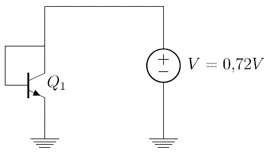
\includegraphics[width=0.3\textwidth]{figuras/ebers_moll_prueba_1.png}\hspace{10mm}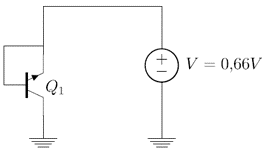
\includegraphics[width=0.3\textwidth]{figuras/ebers_moll_prueba_2.png}

    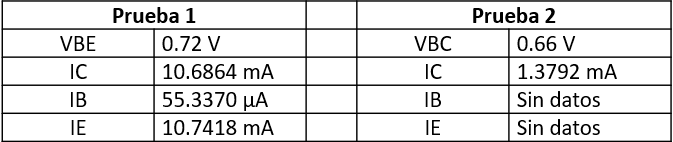
\includegraphics[width=0.7\textwidth]{figuras/ebers_moll_prueba_3.png}
\end{figure}

Con base en la información de las tablas, determine los siguientes parámetros del modelo de Ebers-Moll: $\alpha_F$, $\beta_F$, $I_{ES}$, $I_{CS}$, $\alpha_R$, $\beta_R$ y calcule los valores de $I_B$ e $I_E$ que se deberían obtener en la prueba 2.



\end{frame}


\begin{frame}{Solución 1: Medición experimental de parámetros de Ebers-Moll}

\begin{columns}
\begin{column}{0.5\textwidth}

Las ganancias de corriente son:
%
\begin{align*}
& \alpha_F = \dfrac{I_C}{I_E} = \dfrac{10.6864\ mA}{10.7418\ mA} = 0.99484 \\
& \beta_F = \dfrac{I_C}{I_B} = \dfrac{10.6864\ mA}{55.3370\ \mu A} = 193.12 \\
\end{align*}

Observe que se cumple que:
%
\begin{align*}
& \alpha_F = \dfrac{\beta_F}{\beta_F + 1} \\
\end{align*}

\end{column}
\begin{column}{0.5\textwidth}

La corriente de subumbral del diodo B-E:
%
\begin{align*}
& I_E = -I_{ES} (e^{V_{BE}/V_t} - 1) + \alpha_R I_{CS} (e^{V_{BC}/V_t} - 1) \\
& I_E = -I_{ES} (e^{V_{BE}/V_t} - 1) \\
& I_{ES} = \dfrac{-I_E}{(e^{V_{BE}/V_t} - 1)} \\
& I_{ES} = \dfrac{-(-10.7418\ mA))}{(e^{0.72\ V/26\ mV} - 1)} \\
& I_{ES} = 1.01032\times{}10^{-14}\ A \\
\end{align*}

\end{column}
\end{columns}

\end{frame}


\begin{frame}{Solución 1: Medición experimental de parámetros de Ebers-Moll}

\begin{columns}
\begin{column}{0.5\textwidth}

La corriente de subumbral del diodo B-C:
%
\begin{align*}
& I_C = \alpha_F I_{ES} (e^{V_{BE}/V_t} - 1) - I_{CS} (e^{V_{BC}/V_t} - 1) \\
& I_C = - I_{CS} (e^{V_{BC}/V_t} - 1) \\
& I_{CS} = \dfrac{-I_C}{(e^{V_{BC}/V_t} - 1)} \\
& I_{CS} = \dfrac{-(-1.3792\ mA))}{(e^{0.66\ V/26\ mV} - 1)} \\
& I_{CS} = 1.304\times{}10^{-14}\ A \\
\end{align*}

\end{column}
\begin{column}{0.5\textwidth}

La ganancia C-E de reversa:
%
\begin{align*}
& \alpha_F I_{ES} = \alpha_R I_{CS} \\
& \alpha_R = \dfrac{\alpha_F I_{ES}}{I_{CS}} \\
& \alpha_R = \dfrac{(0.99484)(1.010\times{}10^{-14}\ A)}{1.304\times{}10^{-14}\ A} \\
& \alpha_R = 0.77088 \\
\end{align*}

La ganancia C-B de reversa:
%
\begin{align*}
& \beta_R = \dfrac{\alpha_R}{1 - \alpha_R} = \dfrac{0.77088}{1 - 0.77088} = 3.36453 \\
\end{align*}


\end{column}
\end{columns}

\end{frame}


\begin{frame}{Solución 1: Medición experimental de parámetros de Ebers-Moll}

\begin{columns}
\begin{column}{0.5\textwidth}

La corriente de base de la prueba 2:
%
\begin{align*}
& I_B = \dfrac{I_C}{\beta_R} = \dfrac{1.3792\ mA}{3.36453} = 409.92\ \mu A \\
\end{align*}

La corriente de emisor de la prueba 2:
%
\begin{align*}
& I_E + I_B + I_C = 0 \\
& I_E = -I_C - I_B \\
& I_E = -(-1.3792\ mA) - (409.92\ \mu A) \\
& I_E = 969.28\ \mu A \\
\end{align*}

\end{column}
\begin{column}{0.5\textwidth}



\end{column}
\end{columns}

\end{frame}


\section{Ejemplo 2}
\begin{frame}{Ejemplo 2: Ebers-Moll para saturación}



\begin{columns}

\begin{column}{0.7\textwidth}

Considere el circuito que se muestra en la figura, donde se conoce de antemano que el transistor está operando en la región de saturación fuerte. 

\vspace{3mm}Los parámetros del modelo de Ebers-Moll son: $\alpha_F=0.99$, $\alpha_R=0.495$, $I_{ES}=1\times{}10^{-17}\ A$, $I_{CS}=2\times{}10^{-17}\ A$. La tensión de alimentación es $V_{CC} = 5\ V$.

\vspace{3mm}
\begin{itemize}
    \item Determine el punto de operación del circuito, considerando que $R_B = 220\ k\Omega$, $R_C = 3\ k\Omega$.
    \item Compruebe el resultado mediante simulación en LTspice.
\end{itemize}

\end{column}

\begin{column}{0.3\textwidth}

\begin{figure}
    \centering
    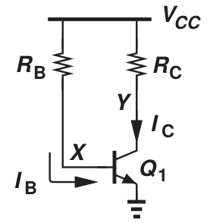
\includegraphics[width=\textwidth]{figuras/ebers_moll_circuito_ejemplo_1.png}
\end{figure}

\end{column}

\end{columns}

\end{frame}


\begin{frame}{Solución 2: Ebers-Moll para saturación}

\begin{columns}

\begin{column}{0.4\textwidth}

\begin{figure}
    \centering
    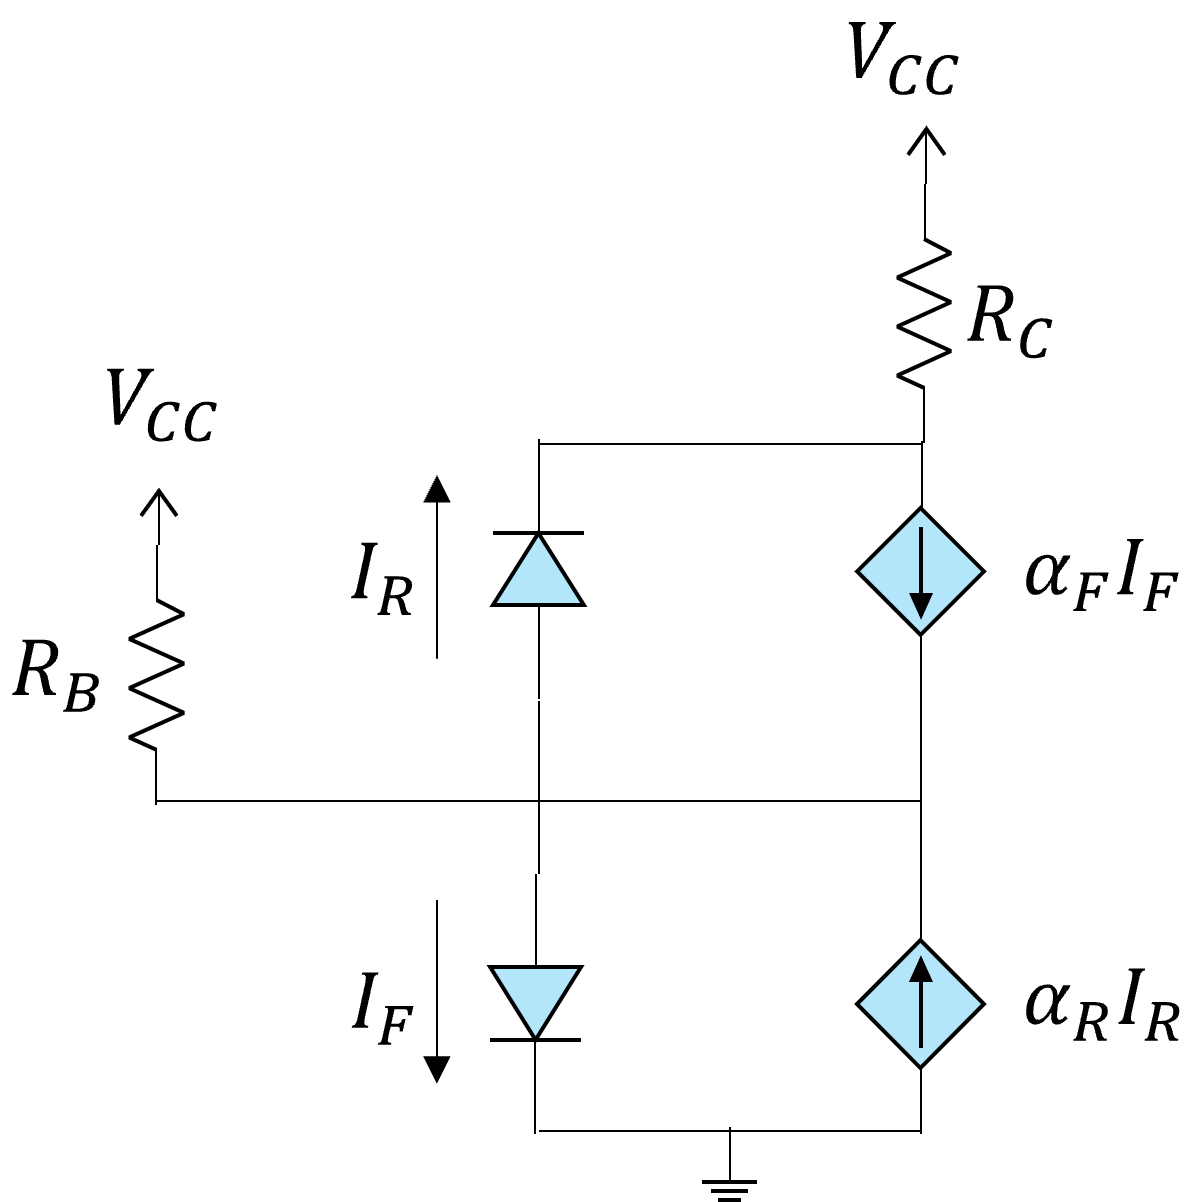
\includegraphics[width=\textwidth]{figuras/ebers_moll_circuito_ejemplo_2.png}
\end{figure}

\end{column}

\begin{column}{0.6\textwidth}

Las ecuaciones de malla del circuito:
\begin{equation*}
\begin{cases}
    V_{CC} = I_B R_B + V_{BE} \\
    V_{CC} = I_C R_C + V_{CE}
\end{cases}
\end{equation*}

La relación de tensiones:
\[ V_{CE} = V_{CB} + V_{BE} \]

Sustituyendo en la segunda:

\begin{equation*}
\begin{cases}
    V_{CC} = I_B R_B + V_{BE} \\
    V_{CC} = I_C R_C + V_{CB} + V_{BE}
\end{cases}
\end{equation*}

\end{column}

\end{columns}

\end{frame}


\begin{frame}{Solución 2: Ebers-Moll para saturación}

\begin{columns}

\begin{column}{0.5\textwidth}

Las relaciones de corriente:
\begin{align*}
&I_B + I_C + I_E = 0 \\
&I_B = - I_C - I_E
\end{align*}

Sustituyendo en la primera:
\begin{equation*}
\begin{cases}
    V_{CC} = (- I_C - I_E) R_B + V_{BE} \\
    V_{CC} = I_C R_C + V_{CB} + V_{BE}
\end{cases}
\end{equation*}

Cambiando el signo de $V_{CB}$ por $-V_{BC}$:
\begin{equation*}
\begin{cases}
    V_{CC} = (- I_C - I_E) R_B + V_{BE} \\
    V_{CC} = I_C R_C - V_{BC} + V_{BE}
\end{cases}
\end{equation*}

\end{column}

\begin{column}{0.5\textwidth}

Las ecuaciones de Ebers-Moll:
\begin{equation*}
\begin{cases}
I_C = \alpha_F I_F - I_R \\
I_E = \alpha_R I_R - I_F
\end{cases}
\end{equation*}

Donde:
\begin{equation*}
\begin{cases}
I_F = I_{ES} (e^{V_{BE}/V_t} - 1) \\
I_R = I_{CS} (e^{V_{BC}/V_t} - 1)
\end{cases}
\end{equation*}

Con las dos ecuaciones del circuito, y las dos ecuaciones del modelo, se puede resolver el sistema de ecuaciones para obtener las cuatro variables.

\end{column}

\end{columns}

\end{frame}



\begin{frame}{Solución 2: Ebers-Moll para saturación}

\begin{columns}

\begin{column}{0.5\textwidth}

Las relaciones de corriente:
\begin{align*}
&I_B + I_C + I_E = 0 \\
&I_B = - I_C - I_E
\end{align*}

Sustituyendo en la primera:
\begin{equation*}
\begin{cases}
    V_{CC} = (- I_C - I_E) R_B + V_{BE} \\
    V_{CC} = I_C R_C + V_{CB} + V_{BE}
\end{cases}
\end{equation*}

Cambiando el signo de $V_{CB}$ por $-V_{BC}$:
\begin{equation*}
\begin{cases}
    V_{CC} = (- I_C - I_E) R_B + V_{BE} \\
    V_{CC} = I_C R_C - V_{BC} + V_{BE}
\end{cases}
\end{equation*}

\end{column}

\begin{column}{0.5\textwidth}

Las ecuaciones de Ebers-Moll:
\begin{equation*}
\begin{cases}
I_C = \alpha_F I_F - I_R \\
I_E = \alpha_R I_R - I_F
\end{cases}
\end{equation*}

Donde:
\begin{equation*}
\begin{cases}
I_F = I_{ES} (e^{V_{BE}/V_t} - 1) \\
I_R = I_{CS} (e^{V_{BC}/V_t} - 1)
\end{cases}
\end{equation*}

Con las dos ecuaciones del circuito, y las dos ecuaciones del modelo, se puede resolver el sistema de ecuaciones para obtener las cuatro variables.

\end{column}

\end{columns}

\end{frame}



\begin{frame}{Solución 2: Ebers-Moll para saturación}

\begin{columns}

\begin{column}{0.5\textwidth}

\begin{figure}
    \centering
    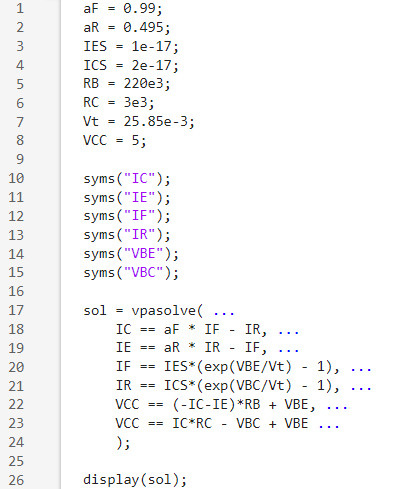
\includegraphics[width=0.7\textwidth]{figuras/solution_1.png}
\end{figure}

\end{column}

\begin{column}{0.5\textwidth}

\begin{figure}
    \centering
    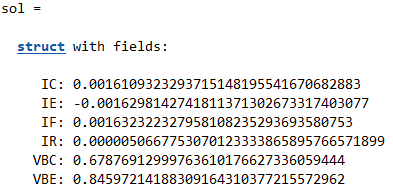
\includegraphics[width=0.8\textwidth]{figuras/solution_2.png}
\end{figure}

Note que la tensión base-colector es \textbf{positiva}, lo cual significa que el colector tiene una tensión menor que la base.

\vspace{5mm}Calcule la tensión en las tres terminales.

\end{column}

\end{columns}

\end{frame}



\begin{frame}{Solución 2: Ebers-Moll para saturación}

\begin{figure}
    \centering
    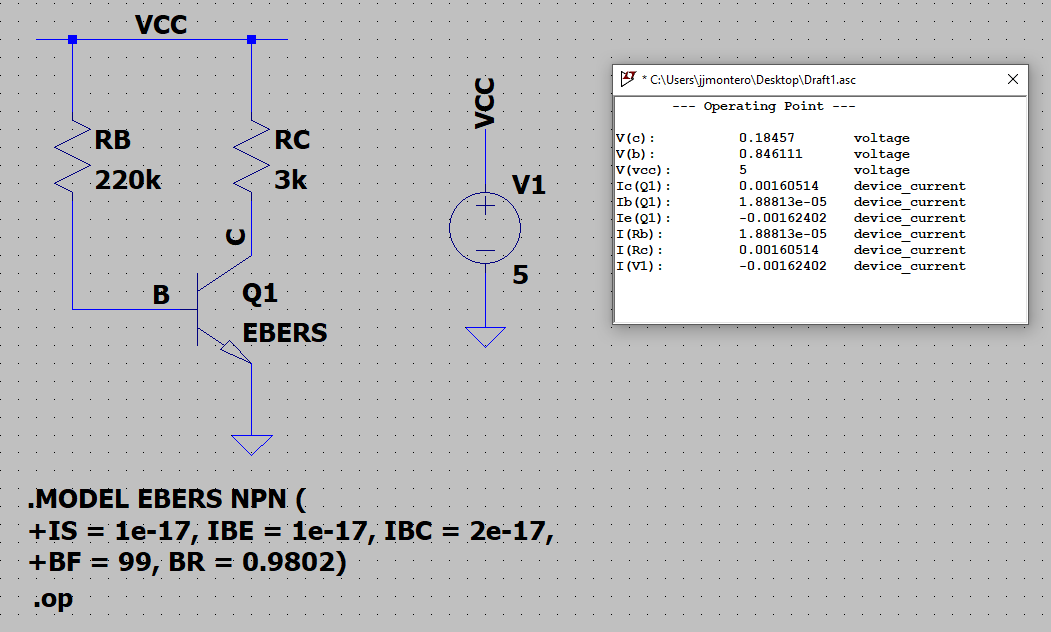
\includegraphics[width=0.8\textwidth]{figuras/solution_3.png}
\end{figure}

\end{frame}


\section{Modelo SPICE}
\begin{frame}{Modelo de SPICE del transistor BJT}

\begin{table}[H]
    \centering
    \begin{tabular}{llll}
        \textbf{Name}    &\textbf{Description}      &\textbf{Units}  &\textbf{Default}    \\
        Is      &Transport saturation current       &A      &1.00E-16   \\
        Ibc     &Base-collector saturation current  &A      &Is         \\
        Ibe     &Base-emitter saturation current    &A      &Is         \\
        Vaf     &Forward Early voltage              &V      &Infin.     \\
        Var     &Reverse Early voltage              &V      &Infin.     \\
        Bf      &Ideal maximum forward beta         &-      &100        \\
        Br      &Ideal maximum reverse beta         &-      &1.         \\
    \end{tabular}
\end{table}


\end{frame}


\section{Referencias}
\begin{frame}{Lecturas recomendadas}

\begin{itemize}
\item Howe, R. and Sodini, C. (1997). Microelectronics, an integrated approach. Chapter 7: The Bipolar Junction Transistor, pp. 410-416, Pearson.
\item Neamen, D. (2011). Semiconductor Physics and Devices: Basic Principles. Chapter 10: The Bipolar Transistor, 3rd ed, pp. 536-540, McGraw-Hill.
\end{itemize}

\end{frame}



\end{document}
